\begin{spacing}{2}
\section{Software in the loop Simulation}
The term ‘software-in-the-loop testing’ is  a test methodology for testing executable codes, algorithms and controller strategies written for a robotic system within a modelling or simulated environment to test the software. Ardupilot, the flight firmware chosen possesses an additional benefit of SITL simulation support which means that actual flight tests are not required in the beginning stages of ROS architecture development and initial testing.\\ SITL allows to run ArduPilot on PC directly, without any special hardware like flight controller. ArduPilot being a portable autopilot can be run on a very wide variety of platforms allowing SITL testing. A personal computer is just another platform on which ArduPilot can be built and run. When running in SITL the sensor data comes from a flight dynamics model in a flight simulator (generally JSBSim). ArduPilot provides a wide range of built in vehicle simulators, and can interface to several external simulators like flight-gear and Xplane. This allows ArduPilot to be tested on a very wide variety of vehicle types. For example, SITL can simulate:
\begin{itemize}
    \item multi-rotor aircraft
    \item fixed wing aircraft
    \item ground vehicles
    \item underwater vehicles
    \item camera gimbals
    \item antenna trackers
    \item optional sensors, such as Lidars and optical flow sensors
\end{itemize}

\noindent Its easy to add a new simulated vehicle type or sensor.
A big advantage of ArduPilot on SITL is it gives access to the full range of
development tools available to desktop C++ development, such as interactive
debuggers, static analyzers and dynamic analysis tools making development and
testing of new features in ArduPilot much simpler.

\subsection{SITL Architecture}
The architecture of the SITL simulation is illustrated in the Fig. \ref{fig:sitlarch}. The
arduplane desktop executable file is used to mimic the controls generated by the
firmware while Physics of Flight Dynamics are handled by JSBSim and FlightGear.
The Ground Control Software used during the SITL simulations is MAVProxy,
however, all telemetry data can be forwarded for interfacing to other GCS.

\begin{figure}
    \centering
    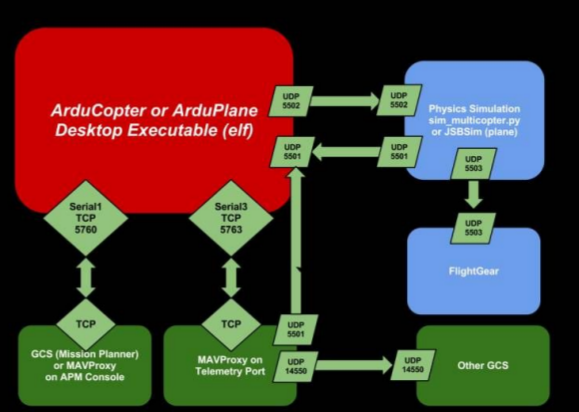
\includegraphics[width=0.8\linewidth]{image/SITLarch.png}
    \caption{Software in the Loop architecture for Ardupilot}
    \label{fig:sitlarch}
\end{figure}

SITL support for Ardupilot was built by the developers for simulating only one
vehicle and hence the architecture needs to be modified in order to run different
instances of SITL on a common computer and make them compatible for swarm
implementation. Some of these changes made to the SITL framework of Ardupilot to
support swarming include:
\begin{itemize}
    \item Shifting of vehicle by a certain offset for each new instance
    \item Assigning a unique MAV\_ID to each vehicle
    \item Change of destination IPs and ports
\end{itemize}
The changes in the SITL framework was followed by creation of a bash script
which takes number of vehicles N and place of origin P as arguments and create N
instances of SITL each shifted by safe distance x around the spawn location P.
Additional telemetry output ports were added in order to visualise all the vehicles
on a common Ground Control Software. MAVLink outputs were also added for MAVROS interfacing. The home location of all the vehicles was kept same using a
pymavlink based script which ensured a common local coordinate system for all the
vehicles, which further reduces the effort of converting the local coordinate system
based codes to global positioning system based coordinate system.
Fig. \ref{fig:sitl instance} and Fig. \ref{fig:qgc} shows a running SITL instance and a group of 3 vehicles connected to a common ground station respectively.

\begin{table}
    \centering
    \caption{SITL Testing Results}
    \begin{tabular}{c|c}
         Parameter &  Value\\\hline
         Maximum Number of vehicles & 10 \\
         Total Flight Hours & 58 \\
         Number of Formations & 6 \\
         Total Missions Performed & 152 
    \end{tabular}
    
    \label{tab:sitlresult}
\end{table}
\begin{figure}
    \centering
    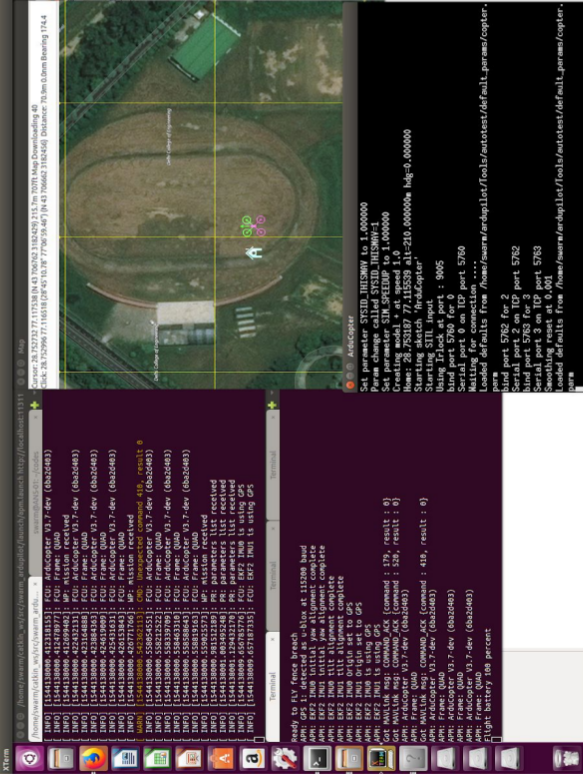
\includegraphics[height = \linewidth, angle=270]{image/sitlscreen.png}
    \caption{Ardupilot SITL instance}
    \label{fig:sitl instance}
\end{figure}
\begin{figure}
    \centering
    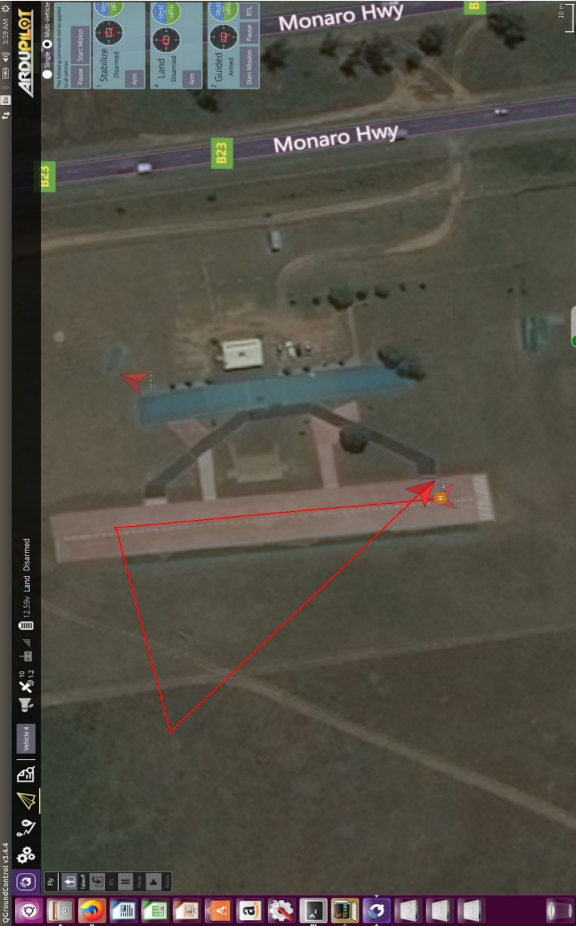
\includegraphics[height = \linewidth, angle=270]{image/sitlmultiUAVQGC.png}
    \caption{Multi-UAV SITL simulation}
    \label{fig:qgc}
\end{figure}
\section{Hardware Testing}
Hardware Testing of aerial swarms was done by using 4 vehicles in both centralized and decentralised manner using different communication systems for data transfer. \\The centralized approach involved transfer of current state of all vehicles to the ground control station where it was analysed and used for generating output for all the vehicles in the swarm. \\ The decentralised approach, on the other hand, used on-board computers and wifi ad-hoc intra-swarm network for exchanging current state information and each vehicle's on-board computer computed the desired output for itself. Fig. \ref{fig:hardwaretest} depicts flight testing of 4 vehicles.
\subsection{Communication Link}
The communication system was tested on ground to ensure reasonable latency at safe distances. A bash script was written to log the latency and the on-board computers tried to ping each other over the ad-hoc network. While addition of new nodes increased the latency initially, the results were negligible after 7 vehicles and the overall system proved to have a latency of less than 150 ms with 9 nodes separated by 10 feet each, providing sufficient margin to avoid collisions despite minor GPS inaccuracies. 

\begin{table}
    \centering
    \caption{Hardware Testing Results}
    \begin{tabular}{c|c}
         Parameter &  Value\\\hline
         Maximum Number of vehicles & 4 \\
         Total Flight Time & 48 mins \\
         Number of Formations & 3 \\
         Total Missions Performed & 7 
    \end{tabular}
    
    \label{tab:flightresult}
\end{table}

\begin{figure}[h]
    \centering
    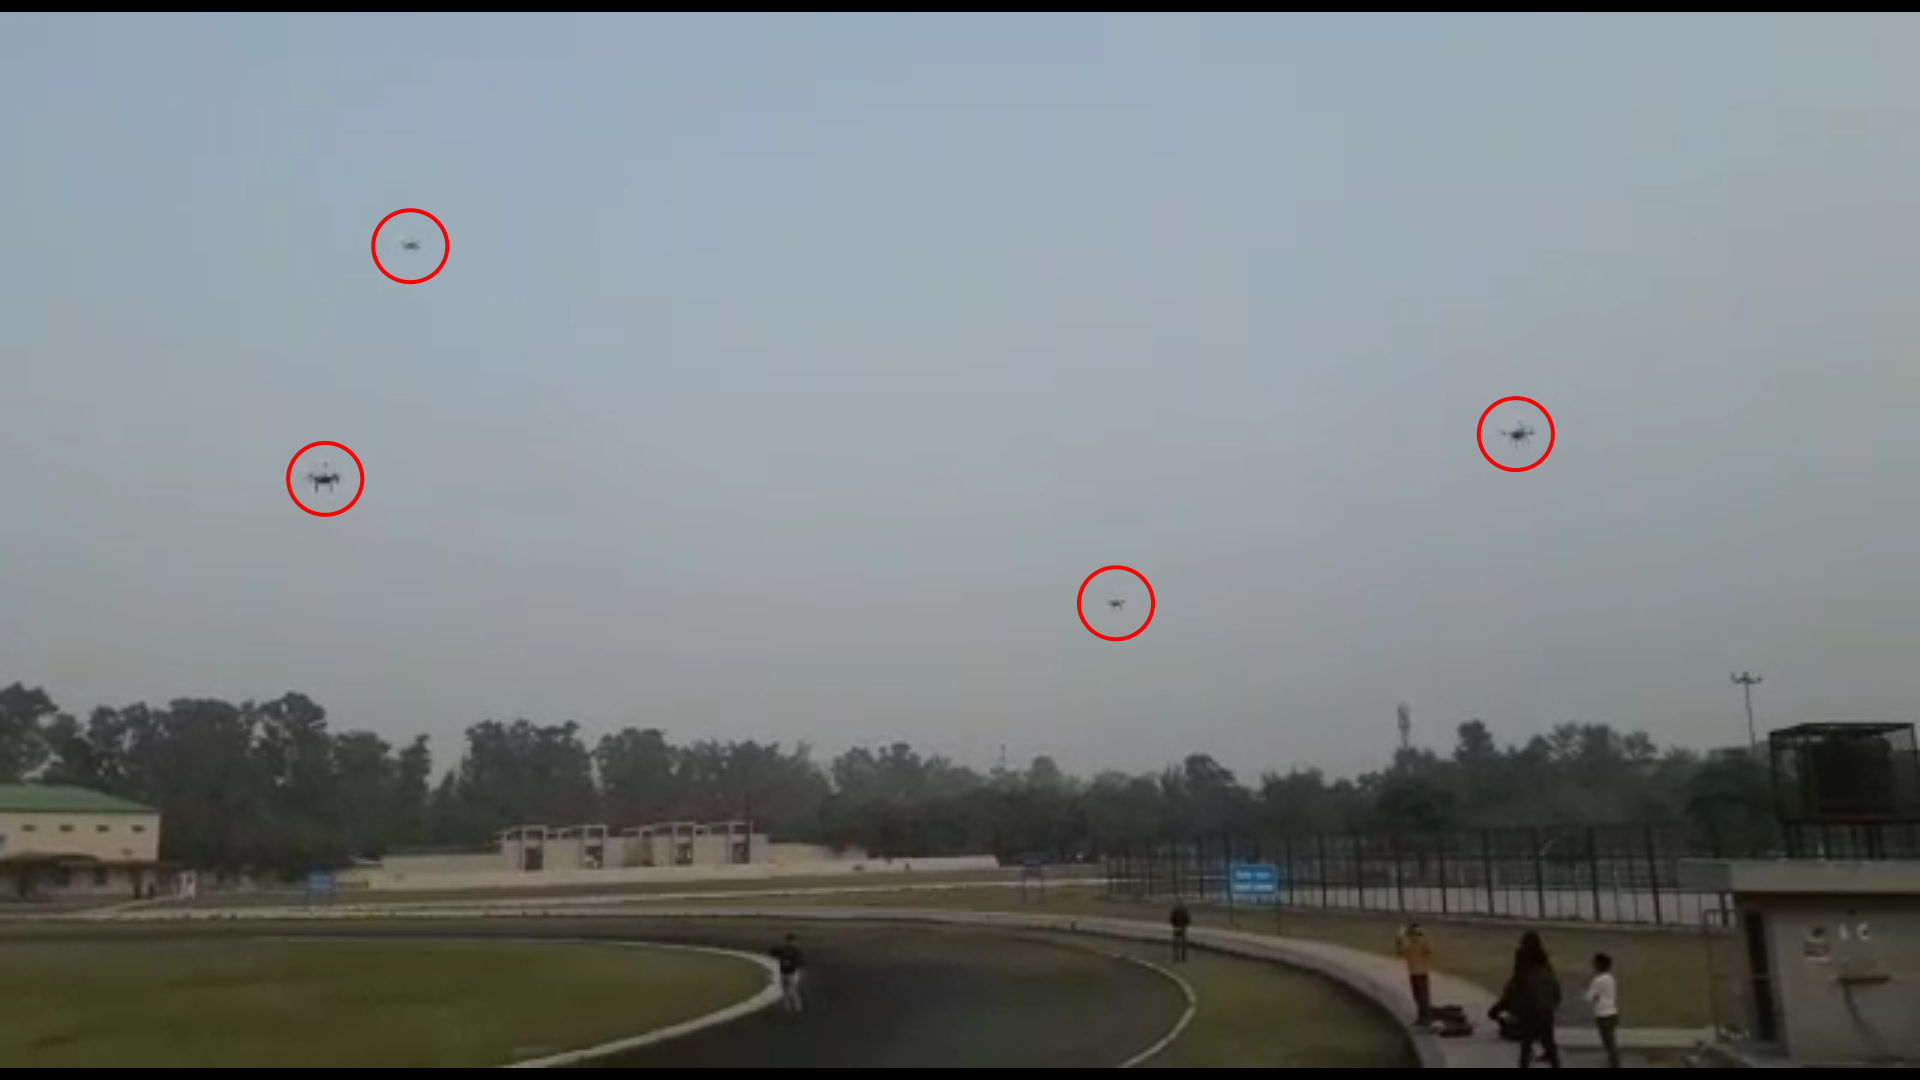
\includegraphics[width=\linewidth]{image/swarm_quad.png}
    \caption{Flight Testing of 4 UAVs implementing aggregation}
    \label{fig:hardwaretest}
\end{figure}

\subsection{Flight Testing}
Various flight tests were conducted with 3 and 4 multi-rotors to achieve flight formations (grid, line and V) using both centralised and decentralised approaches. A total of 3 crashes were observed due to less safety margin and latency observed in centralised communication approach. The data for the conducted hardware testing is given in \ref{tab:flightresult}.

\end{spacing}